\documentclass[twocolumn]{article}
\usepackage{latexsym}
\usepackage{amsmath, amsthm, amssymb}
\usepackage{url}
\usepackage{graphicx}

\usepackage[spanish]{babel}
\usepackage[utf8]{inputenc}
\setlength{\textheight}{8.75in}
\setlength{\columnsep}{2.0pc}
\setlength{\textwidth}{6.8in}
\setlength{\topmargin}{0.25in}
\setlength{\headheight}{0.0in}
\setlength{\headsep}{0.0in}
\setlength{\oddsidemargin}{-.19in}
\setlength{\parindent}{1pc}

\makeatletter
%as Latex cosiders descenders in its calculation of interline spacing, 
%to get 12 point spacing for normalsize text, must set it to 10 points 
\def\@normalsize{\@setsize\normalsize{10pt}\xpt\@xpt
\abovedisplayskip 10pt plus2pt minus5pt\belowdisplayskip \abovedisplayskip 
\abovedisplayshortskip \z@ plus3pt\belowdisplayshortskip 6pt plus3pt 
minus3pt\let\@listi\@listI}
%need an 11 pt font size for subsection and abstract headings 
\def\subsize{\@setsize\subsize{12pt}\xipt\@xipt}
%make section titles bold and 12 point, 2 blank lines before, 1 after 
\def\section{\@startsection {section}{1}{\z@}{1.0ex plus 1ex minus
 .2ex}{.2ex plus .2ex}{\large\bf}}
%make subsection titles bold and 11 point, 1 blank line before, 1 after 
\def\subsection{\@startsection {subsection}{2}{\z@}{.2ex plus 1ex} 
{.2ex plus .2ex}{\subsize\bf}}
\makeatother


\begin{document} 

\title{\Large\bf Visualizaci\'{o}n del mercado de acciones en 3D }
\author{Juan E. Pemberthy, Juan S. Muñoz, Juan G. Lalinde \\
  \textit{Departamento de Ingeniería de Sistemas} \\
  \textit{Universidad EAFIT} \\
  \textit{Medellin, Antioquia, Colombia} \\
  \textit{\{jpembert, jmunozar, jlalinde\}@eafit.edu.co}}
\date{\today}

\maketitle

\subsection*{\centering Abstract}
{\em
\vspace{5 mm}

El análisis de datos siempre ha estado ligado a una representación gráfica de los mismos, y el mercado de acciones no es la excepción, generalmente para representar éstos datos, los que describen el estado y movimiento en el tiempo de una acción se han utilizado gráficos en segunda dimensión como barras, tortas, entre otras.\\

Esta tesis introduce un nuevo paradigma de visualización en este campo, al pasar de gráficos en dos dimensiones, a una nueva propuesta de contenidos para visualizar los datos en tres dimensiones, permitiéndole a una persona visualizar de una manera innovadora el estado y movimiento de las acciones sobre las que lleve algún tipo de registro.
}

\vspace{8 mm}

\subsection*{Palabras Claves}
\vspace{5 mm}

Bolsa de Valores de Colombia, Mercado Accionario, Acciones, Tesis, Visualización de datos, 3D, Web 2.0.

\vspace{8 mm}
\section{Introducción}
Durante la evolución de la computación moderna se han presenciado avances significativos en los diferentes campos que componen la misma, uno de estos campos es la visualización de aplicaciones, es decir la forma en la que una aplicación es desplegada para que una persona interactue con una máquina con el fin de cumplir una determinada tarea, el surgimiento de la computación gráfica como área de estudio le ha significado a la computación una nueva vía para desarrollar aplicaciones en las que la visualización juega un papel fundamental y que antes apenas si eran soñadas.\\

Con éste proyecto de grado se busca aprovechar la capacidad tecnológica actual para desarrollar contenidos en tercera dimensión que puedan ser visualizados desde cualquier lugar, el tema sobre el que se trabajó fue el movimiento del mercado de acciones Colombiano, se eligió este sector para brindarle a los propietarios de acciones que no están sumergidos de lleno en este mundo una herramienta que les permita identificar fácil y gráficamente el movimiento del mercado, pues actualmente muchas de estas personas llevan control de sus inversiones en un papel, o en un archivo plano, sobre el que construyen una tabla, y/o gráficas limitadas a dos dimensiones.\\
	
Las gráficas en segunda dimensión, son simples y fáciles de entender cuándo se están comparando acciones en una unidad de tiempo ó se esta viendo el movimiento de una sola acción en un período determinado, pero a la hora de comparar varias acciones en un período, una gráfica en 2D podría ser difícil de entender para un usuario común, mientras que una gráfica en 3D facilita el entendimiento de la misma, con el fin de apoyar el problema definido anteriormente, en esta aplicación se diseñaron un conjunto de contenidos en tercera dimensión que recrean la actividad del mercado, dichos contenidos son alimentados desde una base de datos que se actualiza constantemente, tanto datos como contenidos 3D fueron integrados en una aplicación web permitiendo que la aplicación sea visualizada desde cualquier lugar en el que se tenga acceso a Internet.\\

\vspace{8 mm}
\section{Sector beneficiado}
\vspace{5 mm}

El Mercado Público de Valores en Colombia ha pasado por muchas etapas y ha sido manejado por diversas instituciones, las cuales nacen y desaparecen con el correr de los años según cambian las necesidades de quienes intervienen en ellas. Tuvo que pasar un siglo desde la creación de la primera bolsa en el país para que apareciera la Bolsa de Valores de Colombia, institución que hoy representa la unificación del Mercado Bursátil.\cite{RePEc:col:000159:003891}\\

Así como en otros sectores, el desarrollo tecnológico ha jugado un papel fundamental para el desarrollo de la bolsa de valores, pues desde sus inicios quienes han estado sumergidos en este mundo, se han valido de la tecnología de momento para llevar control de las acciones, es así como desde que se presentó una fiebre de especulaciones surgida por las oscilaciones de la tasa de cambio ocurridas a principio de siglo(debido a la guerra de los mil días) y que se desarrollaban todas las noches de 7:00 a 10:00 en el atrio de la catedral de la Candelaria de Medellín y dentro del parque Pedro Justo Berrio\cite{RepEEc:col:piedrahita}, posteriormente culminaban con el desarrollo de negocios en oro y los registros eran calculados con una máquina sumadora o en algunos casos eran parte de un calculo mental. Actualmente la Bolsa cuenta con avanzados sistemas de información de uso interno que permite conocer el estado en tiempo real de una acción y ver como se ha comportado en el tiempo, las personas naturales que poseen acciones y que no tienen acceso a estos sistemas pueden consultar el estado de sus inversiones en diversos sitios públicos (sitios web, revistas, periódicos), en donde se les muestra una información plana a veces acompañada de unos gráficos en dos dimensiones.\\

Muchas de las personas naturales mencionadas anteriormente, llevan el control de sus inversiones en libros y hojas de cálculo diseñadas por ellos mismos, algunos, los mas familiarizados con herramientas tecnológicas utilizan herramientas disponibles (Google Finance entre otras), estas ultimas herramientas son útiles a la hora de llevar el historial y permiten calcular fácilmente ganancias/pérdidas, algunos de los problemas que tienen estas aplicaciones son: 
\begin{enumerate}
\item Los gráficos a pesar de que son claros, están limitados a presentar en dos dimensiones múltiples indicadores, que a la larga le podría representar al usuario común complicaciones a la hora de entender el gráfico.
\item La mayoría no permiten llevar el control personalizado del portafolio, y aquellas que integran esta característica rara vez incluyen a la bolsa de valores de Colombia o son de libre acceso.
\item Ninguna de estas aplicaciones ofrece un componente 3D que permita comparar varias variables que afectan el mercado accionario para apreciar mejor el comportamiento de las acciones, y que aparte de esto se puedan acceder desde un navegador web, pues la tendencia en 3D es desarrollar aplicaciones tipo \textbf{Stand-Alone}\footnote{Aquellos programas que no necesitan de un interpretador para ser ejecutados en una máquina.}
\end{enumerate}

Es por esto que es pertinente el desarrollo de una aplicación que sea portable y permita ser visualizada desde cualquier lugar en cualquier plataforma, ademas de esto que permita apreciar las variables que afectan el mercado accionario Colombiano.

\vspace{8 mm}
\section{Solución}
\vspace{5 mm}

Teniendo clara una necesidad y/o problema a suplir/solucionar, se analizaron varias tecnologías y patrones de desarrollo que permitirían llevar a cabo el desarrollo de una aplicación web, en la que fuera posible visualizar contenidos en 3D que fueran alimentados por una Base de Datos.\\

Las herramientas seleccionadas fueron, \textbf{Ruby on Rails}\footnote{http://rubyonrails.org/} para desarrollar la aplicación web, pensando en un metodología ágil de desarrollo, y que a su vez permitiera que los contenidos fueran fáciles de integrar, el motor de bases de datos elegido fue \textbf{MySql}, por otro lado, se elegió \textbf{Unity3D}\footnote{http://unity3d.com/} por su capacidad de generar contenidos 3D que se apoyan directamente de las tarjetas aceleradoras de video para visualizar dichas escenas, además cuenta con una API que facilita exportar contenidos para que sean visibles en un navegador.\\

\subsection{¿Cómo se complementan estas dos tecnologías?}
\vspace{5 mm}

\emph{Rails} y \emph{Unity3D} son herramientas sobre las que se puede desarrollar efectivamente tanto aplicaciones Web convencionales, así como aplicaciones 3D, pero era necesario que ambas tuvieran la forma de recibir y enviar mensajes a través de un protocolo de comunicación, de tal manera que fuera transparente una llamada de una aplicación a la otra como si se tratase de una llamada local.\\

Dicho protocolo de comunicación, fue soportado por \textbf{Javascript} puesto que \emph{Rails} cuenta con una librería bien soportada para convertir datos nativos de \emph{Ruby} a \emph{Javascript} y ya que el contenido generado por \emph{Unity3D} tiene una API accequible escrita en \emph{Javascript} para controlar el estado del contenido dentro del browser, haciendo entonces a \emph{Javascript} la herramienta óptima para comunicar ambas tecnologias.

\vspace{8 mm}
\section{Desarrollo de la aplicación}
\vspace{5 mm}
\subsection{Desarrollo web}
\vspace{5 mm}

A continuación se describe detalladamente el proceso de construcción que se utilizó para el desarrollo de la aplicación web, seguiendo el estándar de \emph{Rails}, se adoptó una metodología ágil\footnote{Es un proceso de desarrollo de software, desarrollado inicialmente por James Martin en 1980. El método comprende el desarrollo iterativo, y la construcción de prototipos, tiende a englobar también la usabilidad, utilidad y la rapidez de ejecución.} buscando velocidad en el desarrollo del producto, así como calidad, pues la aplicación supliría las necesidades de los usuarios y se entregaría en un tiempo acorde según los límites de tiempo del proyecto.

\subsubsection{Especificaciones.}

El primer paso para desarrollar apropiadamente una aplicación guiada por tests(\emph{Test Driven Development - TDD}), es definir las especificaciones que determinan el comportamiento del sistema, dichas especificaciones más tarde se convertirán en la base de los tests para el desarrollo de la aplicación.\\

En este punto, se describió la aplicación Web a ser escrita teniendo en cuenta la definición del problema y el marco referencial, la tarea principal entonces sería integrar datos con contenidos para lograr el desarrollo final de la aplicación, después de tener claro la necesidad a cubrir y de que se necesitaba brindar un ambiente de fácil acceso y manipulación para los usuarios, se decidió desarrollar una aplicación web con las siguientes especificaciones(especificaciones que mas tarde se ampliarían para la construcción de los test.):


\begin{itemize}
\item[$\bullet$] Sistema de usuarios protegido por contraseña.
\item[$\bullet$] Cada usuario puede registrar un portafolio.
\item[$\bullet$] Cada portafolio esta compuesto por títulos.
\item[$\bullet$] Los títulos representan el estado personal de una acción registrada por el usuario, para de esa manera determinar, si la inversión le representa a su propietario una perdida o una ganancia.
\item[$\bullet$] Dentro del portafolio se pueden agregar, actualizar, comparar y eliminar títulos.
\item[$\bullet$] Cada título puede ser seleccionado para inspeccionar su comportamiento durante un rango de tiempo determinado por el usuario.
\item[$\bullet$] Los títulos de cada usuario pueden ser comparados simultáneamente con el apoyo de los contenidos 3D.
\item[$\bullet$] Los títulos se basan en la información que se obtiene al actualizar las acciones.
\item[$\bullet$] Las acciones se actualizan cada veinte minutos cuándo el mercado esta abierto.
\item[$\bullet$] La página principal no necesita registro, evidencia el comportamiento del mercado con una gráfica en 3D y muestra el estado actual de cada acción.
\end{itemize}

\subsubsection{Definición de modelos.}
\vspace{5 mm}

Con el comportamiento de la aplicación claro, era necesario entonces definir los datos con los que la misma trabajaría, que tablas se necesitarían, que campos, y que tipos de datos estarían siendo manipulados por la aplicación, y cuáles  alimentarían los contenidos 3D.\\

Aparte de los definición de los modelos involucrados, se buscaba estar en la capacidad de trabajar bajo un patrón \textbf{ActiveRecord}\footnote{Es un enfoque al problema de acceder a los datos de una base de datos. Una fila en la tabla de la base de datos se envuelve en una clase, de manera que se asocian filas únicas de la base de datos con objetos del lenguaje de programación usado. Cuando se crea uno de estos objetos, se añade una fila a la tabla de la base de datos. Cuando se modifican los atributos del objeto, se actualiza la fila de la base de datos. La clase envoltorio implementa métodos de acceso para cada columna de la tabla o vista.} pensando en un enfoque \textbf{ORM} que permitiera manipular los registros de la base datos como si se trataran de objetos definidos en el lenguaje de programación \emph{Ruby}.\\

El modelo entidad relación final, y que representa la estructura de la base de datos de la aplicación es el que se muestra en la Figura \ref{fig:erd}, según la información recogida de las especificaciones, era claro que se necesitaba un modelo que representara los usuarios, a su vez dichos usuarios tienen relacionado un portafolio(relación \emph{1..1}), cada portafolio actúa como contenedor de títulos(relación \emph{1..n}), indirectamente entonces, el usuario posee títulos, como sucede en la vida real, el modelo \emph{stock\_action} representa la acción real en el mercado, y sobre la cual existen múltiples títulos asociados.

\begin{figure}[h]
	\centering
		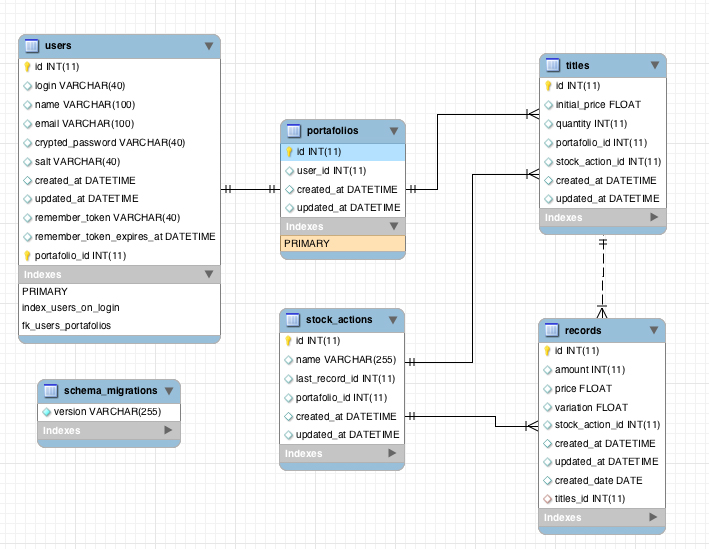
\includegraphics[scale=0.35]{erb_mertd.jpg}
		\caption{Modelo Entidad Relación - Mertd(Mercado 3D)}
	\label{fig:erd}
\end{figure}

Finalmente el modelo \emph{record} es sobre el cual se registran todos los movimientos de las acciones, es decir, sobre el que se hacen las actualizaciones según el estado de una acción, por ejemplo, cada vez que se obtiene información nueva indicando el estado de una acción, un registro nuevo es agregado y guardado en este modelo, luego este registro es usado por otros modelos para calcular el estado de una inversión de forma personalizada.\\

\subsubsection{Servidor Web - \emph{Clusters}}

En el lado de los servidores, se eligió \textbf{Mongrel}\footnote{Es una libreria HTTP y un servidor web para aplicaciones escritas en \emph{Ruby}. Una característica de \emph{Mongrel} es que usa HTTP plano, en vez de \emph{FastCGI} ó \emph{SCGI}, para comunicarse con otros servidores que podrían estar una capa encima de éste.}, encargado de correr la aplicación web a modo de \emph{clusters},\footnote{Los \emph{Mongrel Clusters} son un conjunto de procesos de \emph{Mongrel} con una configuración común que pueden ser manejados por un servidor \emph{Proxy}} éstos interpretan directamente el código escrito en \emph{Ruby} y responden a peticiones HTPP, cuándo se utiliza este esquema se necesita incluir un \textbf{Proxy Sever}\footnote{Es un servidor que intercepta las conexiones de red que un cliente hace a un servidor de destino para actuar como enrutador.} en la primera capa del servidor web, encargado de enrutar las peticiones HTTP a un determinado \emph{cluster} dependiendo del estado de los mismos, para el desarrollo de la aplicación se eligió \textbf{Nginx}\footnote{http://nginx.net/} como servidor proxy.\\

\subsubsection{Daemon - \emph{Stock Getter}}

Al ser una aplicación que necesita estar constantemente recolectando datos desde sitios externos, se hizo necesario la implementación de un Demonio ó \textbf{Daemon} que desarrollara esta tarea, pues una implementación dentro de la aplicación web, al estar corriendo en un mismo proceso, representaría un saturamiento innecesario que podría repercutir en el rendimiento de la aplicación al procesar peticiones HTTP y consecuentemente en la experiencia del usuario.\\

El \emph{Daemon}, se encarga entonces, de recolectar datos nuevos cada 20 minutos mientras que el mercado accionario se encuentre abierto, dicho mercado esta abierto, de Lunes a Vierns de 09:00am a 01:00pm en zona horaria Colombiana (GMT -5), una vez el mercado cierra, el \emph{Daemon} determina la próxima fecha en que el mercado abrirá, calcula los segundos desde el momento actual hasta esa fecha, y entra en estado `dormido' hasta que el mercado vuelva a abrir, y se repita la tarea cada 20 minutos.\\

A continuación se muestra la definición del \emph{Daemon} que recoge los nuevos registros para las acciones en la aplicación. (cabe anotar que se ejectua como un proceso independiente de la aplicación y automatizado.)

\scriptsize
\begin{verbatim}
#!/usr/bin/env ruby
require File.expand_path(File.dirname(__FILE__)) + '/../config/boot' 
rails_root = File.expand_path RAILS_ROOT

ENV["RAILS_ENV"] ||= "production"

Dir.chdir(rails_root) # Change current directory to RAILS_ROOT 
require "config/environment" # Start up rails
require "stock.rb" #loads the stock library.

$running = true
Signal.trap("TERM") do 
  $running = false
end

while($running) do
  #makes work the production logger
  #for debuggin purposes.
  RAILS_DEFAULT_LOGGER.auto_flushing = 1
  s = Stock.new
  col_time = s.time #gets the current colombian time

  if s.open?
    #Hopefully using this statement we dont have to use a monitor.
    ActiveRecord::Base.connection.reconnect!
    s.parsing
    sleep 1200 #1200 secs = 20 mins.
  else
    if(col_time > s.close_time)
      Record.delete_last_history_day(s)
      ActiveRecord::Base.logger.info( 
	          "Deleting last day records, last day => #{s.last_day}")
    end
    ActiveRecord::Base.logger.info "Sleeping at #{col_time}.\n"
    RAILS_DEFAULT_LOGGER.auto_flushing = 1000
    sleep s.secs_til_open #sleeps til next open day.
  end

end
\end{verbatim}
\normalsize

\vspace{8 mm}
\subsubsection{\emph{TDD Cycle}}
\vspace{5 mm}

Siguiendo una metodología como \textbf{TDD}(\emph{Test Driven Development} ó Desarrollo Guiado por Pruebas) se realizó el desarrollo del núcleo de la aplicación, esta práctica de programación se usa generalmente para lograr un código limpio y funcional, la idea es que se utilicen las especificaciones/requerimientos definidos anteriormente, para que sean traducidos en pruebas, cada vez que el conjunto de pruebas que definen un requerimiento pasan, se garantiza que la especificación ha sido implementada correctamente\cite{579193}\cite{864016}. Otro punto importante, es el de hacer pruebas pequeñas con el fin de determinar bajo que condiciones se introduce un error, ó cuando falla la aplicación.\\

El ciclo entonces consiste en que para cada especificación, se debe:
\begin{enumerate}
\item Escribir el test antes de la implementación.
\item Escribir la implementación.
\item Correr el conjunto de tests.
\item Corregir errores en caso de que la prueba falle, de otro modo, avanzar a la siguiente especificación.
\end{enumerate}


\subsection{Desarrollo Contenidos 3D}
La arquitectura dentro de una escena en \textbf{Unity3D} consiste en un conjunto de \textbf{GameObjects} que interactúan entre si para mostrar un evento/animación en una escena; Dichos objetos se comunican, basándose en una jerarquía de objetos, donde la traslación/rotación/escalamiento de un padre afecta directamente a los hijos Figura\ref{fig:jerarq}.\\


\begin{figure}[h]
	\centering
		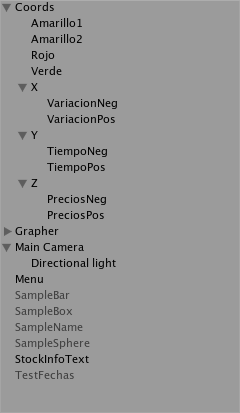
\includegraphics[scale=0.3]{parenting.png}
		\caption{Jerarquía de Objetos en Unity3D.}
	\label{fig:jerarq}
\end{figure}

En este caso, si se rotara/escalára/moviera el objeto `Coords', a su vez a los objetos que se encuentran dentro de `Coords' también se les aplicaría la transformación.\\

Se decidió entonces dividir el programa en 3 grandes módulos principales para facilitar tanto desarrollo como mantenimiento de los contenidos 3D, Dichos modulos le envian información a los otros para renderizar los contenidos 3D. Figura\ref{fig:modules}\\

\begin{figure}[h]
	\centering
		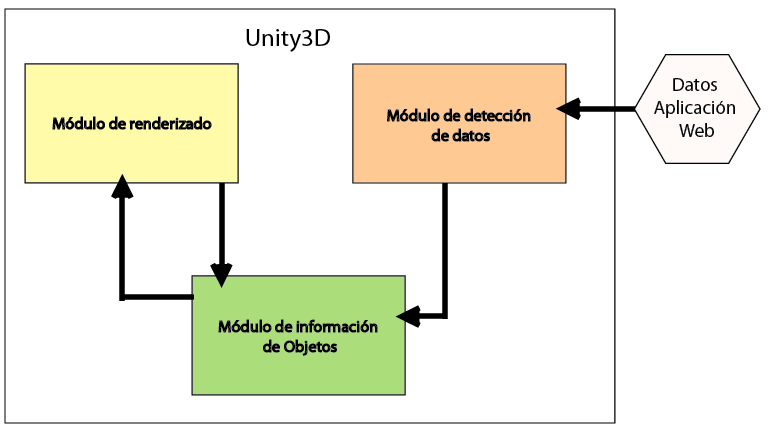
\includegraphics[scale=0.3]{ArquitecturaUnity.png}
		\caption{Arquitectura de los contenidos 3D}
	\label{fig:modules}
\end{figure}


\subsubsection{Módulo de detección de datos e información del exterior:}
Este módulo se encarga de recibir la información que tiene cada acción que proviene desde la aplicación Web parseándola y organizándola para que los otros módulos de la aplicación la entiendan; posteriormente carga en memoria dicha información para así utilizarla apropiadamente en el tipo de gráfico que se esta renderizando.\\

Este módulo solo es usado cada vez que se le inyectan datos a los contenidos 3D ó cada vez que el usuario pide cambiar el tipo de gráfica a mostrar.\\

\subsubsection{Modulo de información de Objetos:}
Este módulo se encarga de recolectar la información almacenada en memoria y cargar para cada objeto que se va a mostrar en la escena, la información pertinente del mismo.\\

Este módulo se encarga del manejo de menús y todo lo que tiene que ver con la interacción del usuario con la aplicación, es llamado constantemente cada vez que el usuario desea averiguar información relevante de una acción, y  se comunica una sola vez con el módulo de detección de datos e información del exterior.\\

\subsubsection{Módulo de renderizado de escena (\emph{Grapher}):}

Finalmente, éste módulo se encarga de lo que es el dibujado de la información proveniente del modulo de información de objetos; éste módulo nunca se entiende con el módulo de datos e información del exterior.\\
 
Para graficar la escena, se recorren todos los nodos que posee el módulo de información y se gráfica (dependiendo del tipo de gráfico) cada nodo\cite{vis:InteractiveVisSmalWorldGraphs}.\\


Cabe aclarar que se debe hacer un `vaciado de hijos' del objeto \emph{Grapher} cada vez que se visualizan contenidos, para no introducir \textbf{leaks}\footnote{Ocurre cuando un bloque de memoria reservada no es liberada en un programa de computación. Comúnmente ocurre porque se pierden todas las referencias a esa área de memoria antes de haberse liberado. Dependiendo de la cantidad de memoria perdida y el tiempo que el programa siga en ejecución, este problema puede llevar al agotamiento de la memoria disponible en la máquina.} de memoria.\\



Basicamente 4 tipos de gráficos fueron los que se decidieron desarrollar: Barras, Espiral, Superficie y el Campo. Cada gráfica ofrece información relevante para cada tipo de variable que se esta analizando. \\

\textbf{Barras} [\ref{fig:Barras}:] Son las típicas barras que se pueden encontrar en cualquier visualización de acciones, pero con el valor agregado de que permiten ver el comportamiento de una o varias acciones a través del tiempo.\\

Estas barras muestran variables como el porcentaje de variación, Cantidad negociada, y Precio; Dichos valores son trabajados de modo percentil para poder comparar las otras acciones que tienen precios diferentes, pues una acción puede valer \$5 mientras que otra puede valer \$20000.\\


\begin{figure}[h]
	\centering
		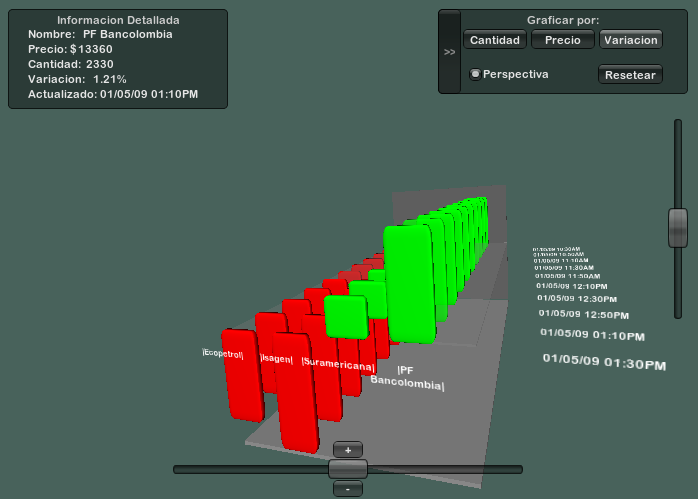
\includegraphics[scale=0.3]{Barras.png}
		\caption{Ejemplo de Visualización por Barras.}
	\label{fig:Barras}
\end{figure}


\textbf{Espiral} [\ref{fig:Espiral}]: Este tipo de gráfica permite comparar rendimientos de varias acciones por medio del porcentaje de variación de cada una en un momento determinado, es el único tipo de gráfico que no permite comparar acciones a través del tiempo, pues lo único que interesa en este gráfico, es determinar de una manera fácil y rápida que acciones están generando mas rentabilidad, cuales están perdiendo y cuales están invariantes en un tiempo dado.\\

\begin{figure}[h]
	\centering
		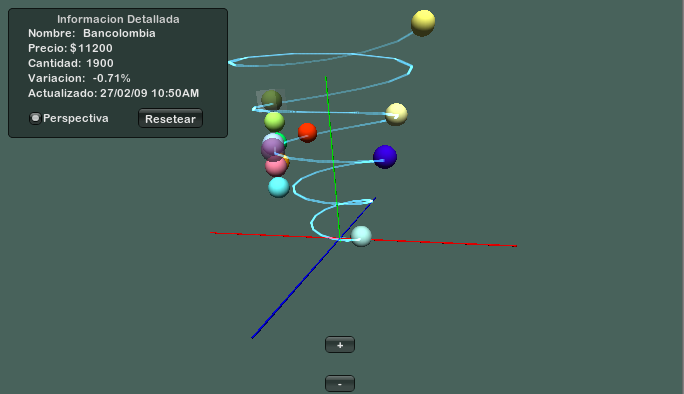
\includegraphics[scale=0.3]{Espiral.png}
		\caption{Ejemplo de Visualización por Espiral.}
	\label{fig:Espiral}
\end{figure}


\textbf{Superficie} [\ref{fig:Superficie}]: Este tipo de gráfico también compara rentabilidades de dos o mas acciones a través del tiempo, con respecto a la mayor/menor rentabilidad de todas las acciones en un momento determinado  mientras que genera una superficie 3D que describe el comportamiento de la bolsa a medida que transcurre el tiempo.\\

\begin{figure}[h]
	\centering
		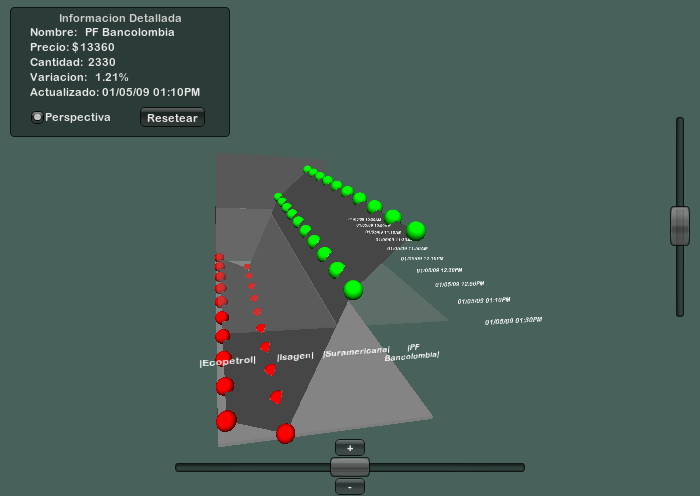
\includegraphics[scale=0.3]{Superficie.png}
		\caption{Ejemplo de Visualización por superficies de rentabilidad.}
	\label{fig:Superficie}
\end{figure}

\textbf{Campo} [\ref{fig:Campo}]: Es el tipo de gráfico mas complejo que se realizó, pues en este gráfico se comparan variables de Cantidad Vs Rentabilidad a través del tiempo\cite{383531}, entonces por medio de estas variables se puede inferir si una acción se esta transando en la bolsa en mucha cantidad o no y si dicha acción esta siendo rentable; Este gráfico provee una serie de `zonas' que ayudan al usuario a entender el estado de las acciones en un momento dado, y así inferir fácilmente si la acción esta generando pérdidas o ganancias y si esta muy o poco demandada\\

\begin{figure}[h]
	\centering
		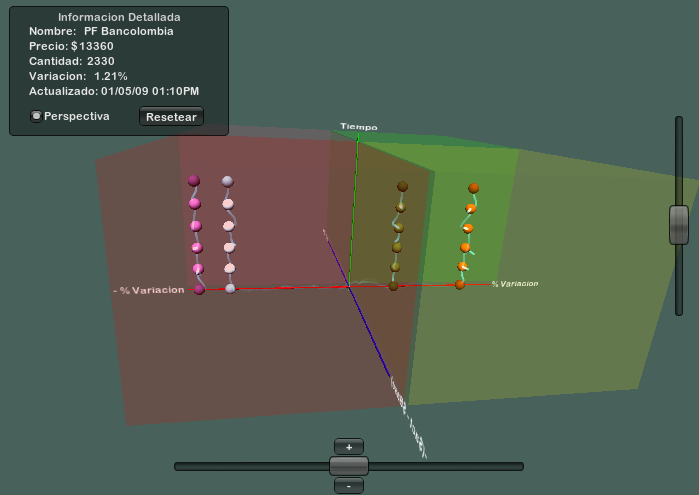
\includegraphics[scale=0.3]{Campo.png}
		\caption{Ejemplo de Visualización por Campos.}
	\label{fig:Campo}
\end{figure}
 

\section{Desarrollo protocolo de comunicación.}

Para el conectar los contenidos 3D con toda la aplicación web, como se mencionó en secciones anteriores, se desarrolló un protocolo escrito en \emph{Javascript}, puesto que \emph{Unity3D} permite el llamado a funciones implementadas dentro del motor por medio de este lenguaje.\\ 

Fue así como por medio de paso de mensajes y llamadas a funciones, se implementó el protocolo de comunicaciones, dicho protocolo actúa como canal sobre el que pasan mensajes a través de funciones nativas de \emph{Javascript} desde la aplicación web (\emph{Ruby} cuenta con una librería especifica para serializar objetos a \emph{Javascript}) a un Objeto \emph{Unity3D} que arroja el \emph{player}, dichas funciónes permiten hacer llamadas nativas a funciones de los contenidos 3D, facilitando este proceso que en un principio pareciera ser más tedioso.\\

El principal problema que se presentó a la hora de diseñar el protocolo fue que el contenido  \emph{HTML} se cargaba antes y mas rápido que el contenido en 3D, lo que conducia eventualmente a la perdida de mensajes y a la incorrecta graficación de los datos. Para solucionar este problema se implementó una llamada desde el contenido 3D a la aplicación web  a través del protocolo que indica cuando un contenido esta listo para recibir datos, y de esta manera graficar correctamente los datos.

A continuación se muestra la parte del protocolo y la función implementada desde el motor, que indica cuando el contenido esta listo para recibir y enviar mensajes.
\scriptsize
\begin{verbatim}
write: function (elementId) {
    if(this.detectUnityWebPlayer()) {
        document.write(this.writeEmbedDOM());
        this.findEar();
        return true;
    } else {
        if(this.getAttribute('altHTML') != "") {
            document.write(this.getAttribute('altHTML'));
        } else if(this.getAttribute('redirectUrl') != "") {
            document.location.replace(
              this.getAttribute('redirectUrl'));
        }
    }
    return false;
},

findEar: function () {
    this.unityEar = "";
    if (navigator.appVersion.indexOf("MSIE") != -1 && 
        navigator.appVersion.toLowerCase().indexOf("win") != -1) {
        this.unityEar = document.getElementById(this.
                                     getAttribute('id')+"_object");
    } else if 
     (navigator.appVersion.toLowerCase().indexOf("safari") != -1) {
        this.unityEar = document.getElementById(this.
                                     getAttribute('id')+"_object")
    } else {
        this.unityEar = document.getElementById(this.
                                     getAttribute('id')+"_embed");
    }
    document.Unity = this.unityEar;
},
   
msg: function (unObj, unFunc, unVar) {
    this.unityEar.SendMessage(unObj, unFunc, unVar);
}
\end{verbatim}
\normalsize
La siguiente porción de código manda una señal hacia el protocolo implementado en \emph{Javascript}, indicando que la aplicación esta lista para renderizar contenidos.\\
\scriptsize
\begin{verbatim}
//Funcion implementada en Unity3D
function Update() {
    if(Application.GetStreamProgressForLevel(0) == 1 && 
       !finishedLoadingApp){
        Application.ExternalCall("FinishedLoadingApp");
        finishedLoadingApp = true;
    }
}
\end{verbatim}
\normalsize

\vspace{8 mm}
\section{Conclusiones}
\vspace{5 mm}

\begin{itemize}

\item[$\bullet$] Se puede aprovechar las nuevas tecnologías de información, las teorías de ambientes virtuales y las ventajas que ofrece la web 2.0 para potenciar el entendimiento del estado actual de las inversiones. De esta forma se puede observar que las plataformas web pueden ser un gran apoyo para llevar a cabo los procesos de visualización, propiciando entornos que no eran imaginados hace unos años atrás.

\item[$\bullet$] Las gráficas 3D son herramientas de toma de decisiones en el mercado bursátil mas poderosas que las convencionales gráficas bidimensionales, ya que estas ofrecen una visión global del movimiento accionario.

\item[$\bullet$] Mejorar la experiencia del usuario en cuanto a interacción con la aplicación puede ser tenido en cuenta en un futuro, pues a medida que se incrementa la facilidad para maniobrar los contenidos, el usuario estará en la capacidad de asimilar más fácilmente los gráficos.

\item[$\bullet$] Las herramientas tecnológicas de visualización + Web2.0 necesitan estar apoyadas en unos lineamientos metodológicos para ayudar a potencializar y agilizar el desarrollo, de otra manera, tener una plataforma que no este testeada o que presente varios problemas, es incurrir en mas esfuerzos y gastos en el proceso de desarrollo

\item[$\bullet$] Aplicar un estándar para el desarrollo de aplicaciones Web 2.0 como el \texttt{TDD} trae grandes ventajas y facilita el manejo y desarrollo de la aplicación, pues de esta forma la misma tendrá unas características mejor desarrolladas en cuanto a reusabilidad, accesibilidad y seguimiento al usuario.

\item[$\bullet$] Antes de desarrollar una aplicación es necesario conocer todo el modelo de negocio de la institución cliente, ya que sin hacer un análisis del entorno es imposible modelar una solución que se adapte a las necesidades específicas y a las características de los usuarios. Del mismo modo, realizar un proceso de planeación previo al desarrollo del producto es importante para distribuir de una forma mejor los recursos disponibles.

\item[$\bullet$] Por medio de la visualización 3D se pueden observar clara y didácticamente los patrones de fluctuación del mercado	

\item[$\bullet$] Utilizar herramientas y plataformas existentes para adaptarlas a las necesidades específicas de la aplicación solicitada trae mucha facilidad, ahorro de tiempo y esfuerzo, pues de esta forma se puede enfocar en las nuevas funcionalidades y en el modelado del problema. En nuestro caso especifico, utilizar y apoyarnos en \emph{Rails} + \emph{Unity3D} para ofrecerle al usuario los servicios requeridos de interacción (Agregar acciones, ganancias diarias, ganancias totales.) fue de gran utilidad porque no fue necesario implementar el sistema desde cero y no se necesitaron crear elementos ya existentes. De esta forma nos pudimos enfocar primordialmente en las necesidades específicas de los jugadores en la bolsa, permitiendo acotar el problema y trayendo finalmente beneficios que se vieron reflejados en el ahorro de tiempo y facilidad de la implementación.	
	
\end{itemize}
\bibliography{article}
\bibliographystyle{plain}

%\bibliographystyle{plain}

\end{document}



